%Every piece of package I've acumulated over the last years
%%%%%%%%%%%%%%%%%%%%%%%%%%%%%%%%%%%%%%%%%%%%%%%%%%%%%%%%%%%%%%%%%%%%%%%%%%%%%%%%%%%%%%%%%%%%%%
\documentclass[a4paper,12pt]{article}
\usepackage[utf8]{inputenc}
\usepackage{imakeidx}
\usepackage{graphicx}
\usepackage{float}
\usepackage{amsmath}
\usepackage[backend=bibtex,style=verbose]{biblatex}
\bibliography{bibliography}
\usepackage{csquotes}
\usepackage{tcolorbox}
\usepackage{multirow}
\usepackage{caption}
\usepackage{afterpage}
\usepackage[margin=1in]{geometry}
\usepackage[english,spanish]{babel}
\usepackage{tikz}
\usepackage{mwe}
\usepackage{circuitikz}
\usepackage{subcaption}
%%%%%%%%%%%%%%%%%%%%%%%%%%%%%%%%%%%%%%%%%%%%%%%%%%%%%%%%%%%%%%%%%%%%%%%%%%%%%%%%%%%%%%%%%%%%%%
\begin{document}
\title{Evaluación Continua de Mecánica II\\ Tema 1}
\author{Gabriel D'Andrade Furlanetto}
\maketitle 

\section{Circuitos LRC acoplados}
En este problema, analizaremos el circuito representado en la Figura \ref{circ} 

\begin{figure}[H]
  \centering
  \caption{Circuito a ser analizado}
  \label{circ}
  \begin{circuitikz}[american voltages]
    \draw
    (0,0) to  [C, l=$C$](2,0)
    to [C, l=$C$] (4,0) 
    to [L, l=$L$] (4,-2)
    to [R, l=$R$] (2,-2)
    to [R, l=$R$] (0,-2)
    to [L, l=$L$] (0,0)
    (2,0) to [L, l=$L$] (2,-2);
  \end{circuitikz}
\end{figure}


\subsection*{a) Escribe las ecuaciones de Kirchoff del circuito y encontra los modos y frecuencias normales.}

Para escribir las ecuaciones de Kirchoff, tenemos que analizar las corrientes utilizando la Ley de Corrientes de Kirchoff, y las tensiones, utilizando la Ley de Voltajes de Kirchoff. El primero es trivial, y está hecho en la Figura \ref{k1}. Para el segundo, utilizaremos las mallas en la Figura \ref{k2}.

\begin{figure}[H]
    \centering
    \begin{minipage}{0.45\textwidth}
        \centering
        \begin{otherlanguage}{english}
        \begin{circuitikz}[american voltages]
          \draw node at (0.45, 0.45) {$I_1$};
          \draw[->] (0.15,0.15)-- (0.75,0.16);
          \draw node at (2.45, 0.45) {$I_2$};
          \draw[->] (2.15,0.15)-- (2.75,0.16);
          \draw node at (1.2, -1) {$I_1-I_2$};
          \draw[->] (1.75,-0.50)-- (1.75,-1.5);
          \draw
          (0,0) to  [C, l=$C$](2,0)
          to [C, l=$C$] (4,0) 
          to [L, l=$L$] (4,-2)
          to [R, l=$R$] (2,-2)
          to [R, l=$R$] (0,-2)
          to [L, l=$L$] (0,0)
          (2,0) to [L, l=$L$] (2,-2);
    \end{circuitikz}
    \end{otherlanguage}
        \caption{Análisis de corrientes}
        \label{k1}
    \end{minipage}\hfill
    \begin{minipage}{0.45\textwidth}
    \begin{otherlanguage}{english}
        \centering
        \begin{circuitikz}[american voltages]
          \draw node at (1,-1) {1};
          \draw node at (3,-1) {2};
          \draw[thick, <-] (1.65,-1) arc (0:320:0.6);
          \draw[thick, <-] (3.65,-1) arc (0:320:0.6);
          \draw
            (0,0) to  [C, l=$C$](2,0)
            to [C, l=$C$] (4,0) 
            to [L, l=$L$] (4,-2)
            to [R, l=$R$] (2,-2)
            to [R, l=$R$] (0,-2)
            to [L, l=$L$] (0,0)
            (2,0) to [L, l=$L$] (2,-2);
    \end{circuitikz}
    \end{otherlanguage}
        \caption{Análisis de mallas}
        \label{k2}
  \end{minipage}
\end{figure}

 Tendremos, finalmente, dos ecuaciones utilizando que $\sum V = 0$ para una malla cerrada. Como $I = \dot{Q}$, seremos capaces de escribir las ecuaciones para la primera y segunda malla, respectivamente:
  \begin{equation}
  \label{eq1}
  \begin{aligned}
  \frac{1}{C} Q_1 + R \dot{Q}_1 + L\ddot{Q}_1 + L(\ddot{Q}_1 - \ddot{Q}_2)) = 0\\
  \frac{1}{C} Q_2 + R \dot{Q}_2 + L\ddot{Q}_2 - L(\ddot{Q}_1 - \ddot{Q}_2)) = 0
  \end{aligned}
  \end{equation}

A este sistema de ecuaciones diferenciales lineales de orden 2 no será posible aplicar las técnicas estándar que desarrollamos durante el curso, ya que tenemos términos con dependencia en las velocidades, o sea, tenemos oscilaciones amortiguadas.

De esta manera, podemos mirar fijamente el Sistema \eqref{eq1} y percibir que si sumamos o tomamos la diferencia de las ecuaciones, podremos trivialmente encontrar unas coordenadas normales (esto es, desacopladas). Es decir, podemos escribir nuestras ecuaciones como:

$$ \frac{1}{C} (Q_1 + Q_2) + R (\dot{Q}_1 + \dot{Q}_2)  + L (\ddot{Q}_1 + \ddot{Q_2})=0 \qquad \text{(Suma)}$$
$$\frac{1}{C} (Q_1 - Q_2) + R (\dot{Q}_1 - \dot{Q}_2) + 3L (\ddot{Q}_1 - \ddot{Q}_2) = 0 \qquad \text{(Sustracción)}$$

Escrito de esa manera, no es un salto de lógica muy grande hacer el siguiente cambio de coordenadas:

\begin{equation}
  \begin{aligned}
    \eta = Q_1 + Q_2 \\
    \xi = Q_1 - Q_2 
  \end{aligned} 
\end{equation}

De manera que tendremos dos osciladores amortiguados desacoplados:

\begin{equation}
\label{coords1}
  \begin{aligned}
    \ddot{\eta} + 2\left(\frac{R}{2L}\right) \dot{\eta} + \left(\sqrt{\frac{1}{CL}}\right)^2 \eta = 0 \\
    \ddot{\xi} + 2\left(\frac{R}{6L}\right) \ddot{\xi} + \left(\sqrt{\frac{1}{3CL}}\right)^2 \xi = 0
  \end{aligned}
\end{equation}

Y podemos encontrar la solución para $\eta$ y $\xi$ por los métodos estándar:
\begin{equation}
\label{coords1}
  \begin{aligned}
    \eta(t) = e^{-\frac{R}{2L}t}\left[A_1 e^{\sqrt{\left(\frac{R}{2L}\right)^2 -\frac{1}{CL}}t} + A_2e^{\sqrt{-\left(\frac{R}{2L}\right)^2 -\frac{1}{CL}}t}\right]\\
    \xi(t) = e^{-\frac{R}{6L}t}\left[A_1 e^{\sqrt{\left(\frac{R}{6L}\right)^2 -\frac{1}{3CL}}t} + A_2e^{\sqrt{-\left(\frac{R}{6L}\right)^2 -\frac{1}{3CL}}t}\right]
  \end{aligned}
\end{equation}

Que no ilumina básicamente nada de nuestro problema.\footnote{Las soluciones tienen más sentido después de ser determinado el régimen de amortiguación}. 

No obstante, solo tendrá sentido hablar de frecuencias normales para el régimen de amortiguamiento débil, ya que es el único que de hecho oscila, y serán definidas por:

\begin{equation}
  \label{eta}
  \omega_{\eta} = \sqrt{\frac{1}{CL} - \left(\frac{R}{2L}\right)^2}
\end{equation}
\begin{equation}
  \label{xi}
  \omega_{\xi} = \sqrt{\frac{1}{3CL} - \left(\frac{R}{6L}\right)^2}
\end{equation}

Es importante mencionar que, una vez encontrados $\eta(t)$ y $\xi(t)$, podemos trivialmente obtener expresiones para $Q_{1}$ y $Q_2$ de la ecuación \eqref{coords1}\footnote{No será muy útil o instructivo hacerlo para las ecuaciones generales de \eqref{eta} y \eqref{xi}, entonces lo haremos solo para el caso particular del apartado siguiente.}:

\begin{equation}
  \begin{aligned}
    Q_1(t) = \frac{\eta(t) + \xi(t)}{2}\\
    Q_2(t) = \frac{\eta(t) - \xi(t)}{2} 
  \end{aligned}
\end{equation}

Finalmente, no es mala idea hacer las analogías que este sistema electrónico tiene a sistemas mecánicos explicita: La decisión de discutir la carga $Q_{i}$ en los capacitores\footnote{Y no corrientes, como se hace usualmente en electrónica} no fue una trivialidad, sino algo que hecho adrede para hacer una conexión estrecha con las coordenadas generalizadas $q_i$. 

De hecho, si se omitiera la primera página de este documento, sería bastante razonable esperar que estuviera resolviendo el problema 25 de la lista de problemas, un oscilador acoplado con un pistón viscoso, representado en la Figura \ref{amort}
\begin{figure}
  \centering
  \caption{Problema 25: Masas-muelles acoplados con pistón viscoso.}
  \label{amort}
  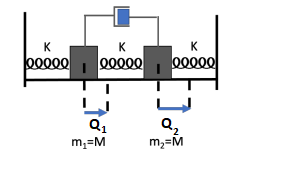
\includegraphics[width=0.5\textwidth]{amort.jpg}
\end{figure}

Fundamentalmente, los métodos de la mecánica clásica no comienzan y acaban en posiciones generalizadas y momentos canónicos, y este problema lo ilustra un poco.

\subsection*{b) Discute los regímenes de amortiguación del circuito. Escribe la solución para el caso particular de $6L = CR^2$}

Algunas generalidades de los regímenes de amortiguación fueron discutidas en la sección anterior, pero fundamentalmente estará dado para cada modo normal por el signo de las cantidades:

$$\Delta_\eta = \left(\frac{R}{2L}\right)^2 - \frac{1}{CL}$$
$$\Delta_\xi = \left(\frac{R}{6L}\right)^2 - \frac{1}{3CL}$$

Si son positivas, tendremos el régimen de sobre-amortiguamiento. Si son 0, tendríamos un amortiguamiento crítico, y si son negativas, tendremos el amortiguamiento débil. Para el caso de $R^2 =\frac{6 L }{C} $, tendremos que:

\begin{equation}
  \Delta_\eta = \frac{R^2}{4 L^2} - \frac{1}{CL} = \frac{6L}{4 L^2 C} - \frac{1}{CL} = \frac{1}{CL} \left(\frac{3}{2} - 1\right) > 0
\end{equation}

Que significa que la coordinada $\eta$ estará sobreamortiguado. Para el otro,

\begin{equation}
  \Delta_\xi = \frac{R^2}{36L^2} - \frac{1}{3CL} = \frac{6 L}{36 L^2 C} - \frac{1}{3CL} = \frac{1}{CL} \left(\frac{1}{6} - \frac{1}{3}\right) < 0
\end{equation}

O sea, la coordinada $\xi$ estará en el régimen de amortiguación débil.

De esta manera, podemos escribir las ecuaciones para los dos:

\begin{equation}
\eta (t) =   e^{-\frac{R}{2L} t}  \left[A_1 e^{\sqrt{\frac{1}{2CL}} t} + B_1 e^{-\sqrt{\frac{1}{2CL}} t}\right]
\end{equation}


\begin{equation}
\xi(t) = e^{-\frac{R}{6CL} t}  A_2\cos{\left(\frac{1}{6CL} t + B_2\right)} 
\end{equation}

Por lo que tenemos que la solución general de nuestro sistema será:

\begin{equation}
  \begin{aligned}
     Q_1(t)& = \eta(t) + \xi(t) \\&= e^{-\frac{R}{2L} t}  \left[A_1 e^{\sqrt{\frac{1}{2CL}} t} + B_1 e^{-\sqrt{\frac{1}{2CL}} t}\right] + e^{-\frac{R}{6CL} t}A_2\cos{\left(\frac{1}{6CL} t + B_2\right)}  
  \end{aligned}
\end{equation}

\begin{equation}
\begin{aligned}
    Q_2(t) &= \eta(t) - \xi(t) \\&= e^{-\frac{R}{2L} t}  \left[A_1 e^{\sqrt{\frac{1}{2CL}} t} - B_1 e^{-\sqrt{\frac{1}{2CL}} t}\right] -e^{-\frac{R}{6CL} t} A_2\cos{\left(\frac{1}{6CL} t + B_2\right)}
\end{aligned}
\end{equation}

Para la corriente, tenemos que derivar estas expresiones. La expresión no son elegantes, pero al final, tendremos que:

\begin{equation}
\begin{aligned}
  I_1(t) =& e^{-\frac{R}{2L} t}  \left[A_1\left(\frac{1}{2CL}- \frac{R}{2L}\right) e^{\sqrt{\frac{1}{2CL}} t} - \left(\frac{1}{2CL}+ \frac{R}{2L}\right)B_1 e^{-\sqrt{\frac{1}{2CL}} t}\right] - A_2 e^{-\frac{R}{6CL} t} \beta\cos{\left(\frac{1}{6CL} t + B_2\right)}\\& + \frac{1}{6CL}\sin{\left(\frac{1}{6CL} t + B_2\right)}
\end{aligned}
\end{equation}

\begin{equation}
\begin{aligned}
  I_2(t) =& e^{-\frac{R}{2L} t}  \left[A_1\left(\frac{1}{2CL}- \frac{R}{2L}\right) e^{\sqrt{\frac{1}{2CL}} t} - \left(\frac{1}{2CL}+ \frac{R}{2L}\right)B_1 e^{-\sqrt{\frac{1}{2CL}} t}\right] + A_2 e^{-\frac{R}{6CL} t} \beta\cos{\left(\frac{1}{6CL} t + B_2\right)}\\& + \frac{1}{6CL}\sin{\left(\frac{1}{6CL} t + B_2\right)}
\end{aligned}
\end{equation}

\pagebreak

\section{ Partículas de masas m en barras fijas con ángulo constante de 2$\alpha$ entre si conectadas con muelles.}
En este problema, analizaremos el sistema mecánico representado en la Figura \ref{2nd}.
\begin{figure}
  \centering
  \caption{Representación del Problema 2}
  \label{2nd}
  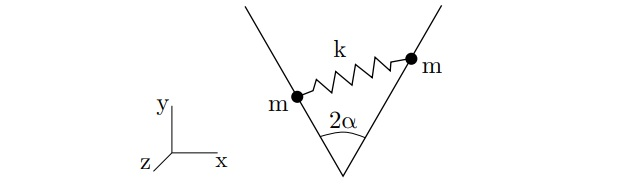
\includegraphics{2.jpg}
\end{figure}

\subsection*{a) Supongamos que hay un campo gravitatorio $g$ en la dirección negativa del eje $y$. Calcula el Lagrangiano, posición de equilibrio, modos y frecuencias normales.}

Para este problema, lo más conveniente es utilizar la distancia del vértice como las coordenadas generalizadas, que llamaremos de $\rho_{1}$ y $\rho_2$. Por algunas relaciones trigonométricas básicas, representadas en la Figura \ref{repr}, tendremos que:

\begin{equation}
  \begin{aligned}
    x_1 = \rho_1 \sin{(\alpha)}\\
    y_1 = \rho_1 \cos{(\alpha)}
  \end{aligned}
\end{equation}
\begin{equation}
  \begin{aligned}
    x_2 = \rho_2 \sin{(\alpha)}\\
    y_2 = \rho_2 \cos{(\alpha)}
  \end{aligned}
\end{equation}

\begin{figure}[h!]
  \centering
  \caption{Representación esquemática del sistema}
  \label{repr}
  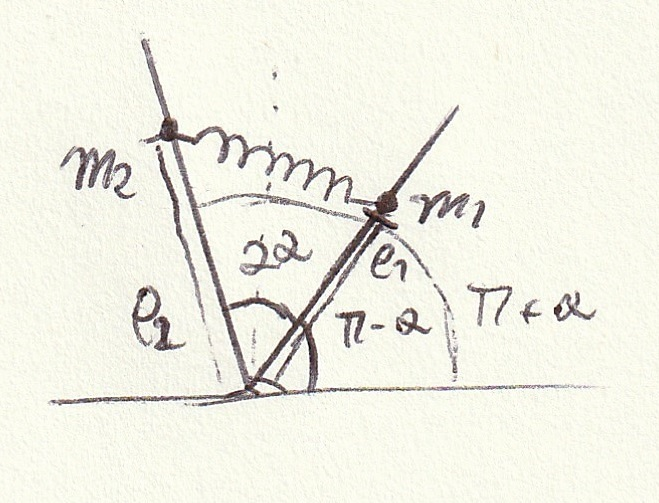
\includegraphics{repr.jpg}
\end{figure}
Trivialmente podemos calcular la energía cinética, que nos saldrá:

\begin{equation}
  T = \frac{1}{2}m (\dot{\rho_1} + \dot{\rho_2})
\end{equation}
Por la presencia de la gravedad, sabemos que la energía potencial tendrá dos términos, uno gravitacional que va a depender de $y_i$ y otro elástico que dependerá de $D$, la distancia entre las masas. Por la ley de cosenos podemos trivialmente calcular esta distancia:

$$D =\sqrt{\rho_1^2 + \rho_2^2 -2\rho_1\rho_2\cos{(2\alpha)}} $$


La energía potencial estará dada por:

$$U = \frac{1}{2}k(D-l_0)^2 + mgy_1+mgy_2 = \frac{1}{2}k \left(\sqrt{\rho_1^2 + \rho_2^2 -2\rho_1\rho_2\cos{(2\alpha)}} - l_0\right)^2 + mg\cos{(\alpha)}\left(\rho_1+\rho_2\right)$$




O sea, nuestro Lagrangiano será:

\begin{equation}
  L = \frac{1}{2}m (\dot{\rho_1} + \dot{\rho_2}) - \frac{1}{2}k (\sqrt{\rho_1^2 + \rho_2^2 -2\rho_1\rho_2\cos{(2\alpha)}} - l_0)^2 + mg\cos{(\alpha)}\left(\rho_1+\rho_2\right)
\end{equation}

Si cambiamos de coordenadas, de modo que $(0,0)$ es el punto de equilibrio de nuestro sistema, será trivial extraer las matrices de masa y de rigidez, que serán respectivamente: 
\begin{equation}
  M = m\begin{pmatrix}
    1&0\\0&1
  \end{pmatrix}
\end{equation}

\begin{equation}
  K = k\begin{pmatrix}
    1&\cos{(2\alpha)}\\\cos{(2\alpha)}&1
  \end{pmatrix}
\end{equation}



\subsection*{c}

En este caso, 
\end{document}

